\begin{figure}[h!]
    \centering
    \caption{Sample of ZIP codes in Zillow data vs.\ population density}
    \label{fig:map_zillow_sample}

    \begin{subfigure}{1\textwidth}
        \centering
        \caption{Zillow ZIP codes}
        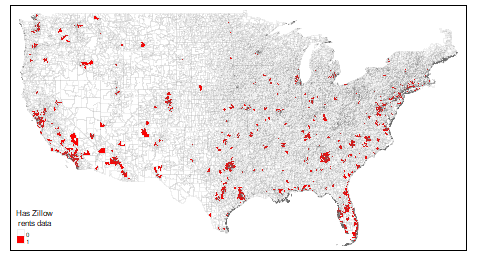
\includegraphics[width = 0.95\textwidth]
            {maps_US/output/USPS_zipcodes_zillow_data.png}
    \end{subfigure}\\
    \begin{subfigure}{1\textwidth}
        \centering
        \caption{Population Density}
        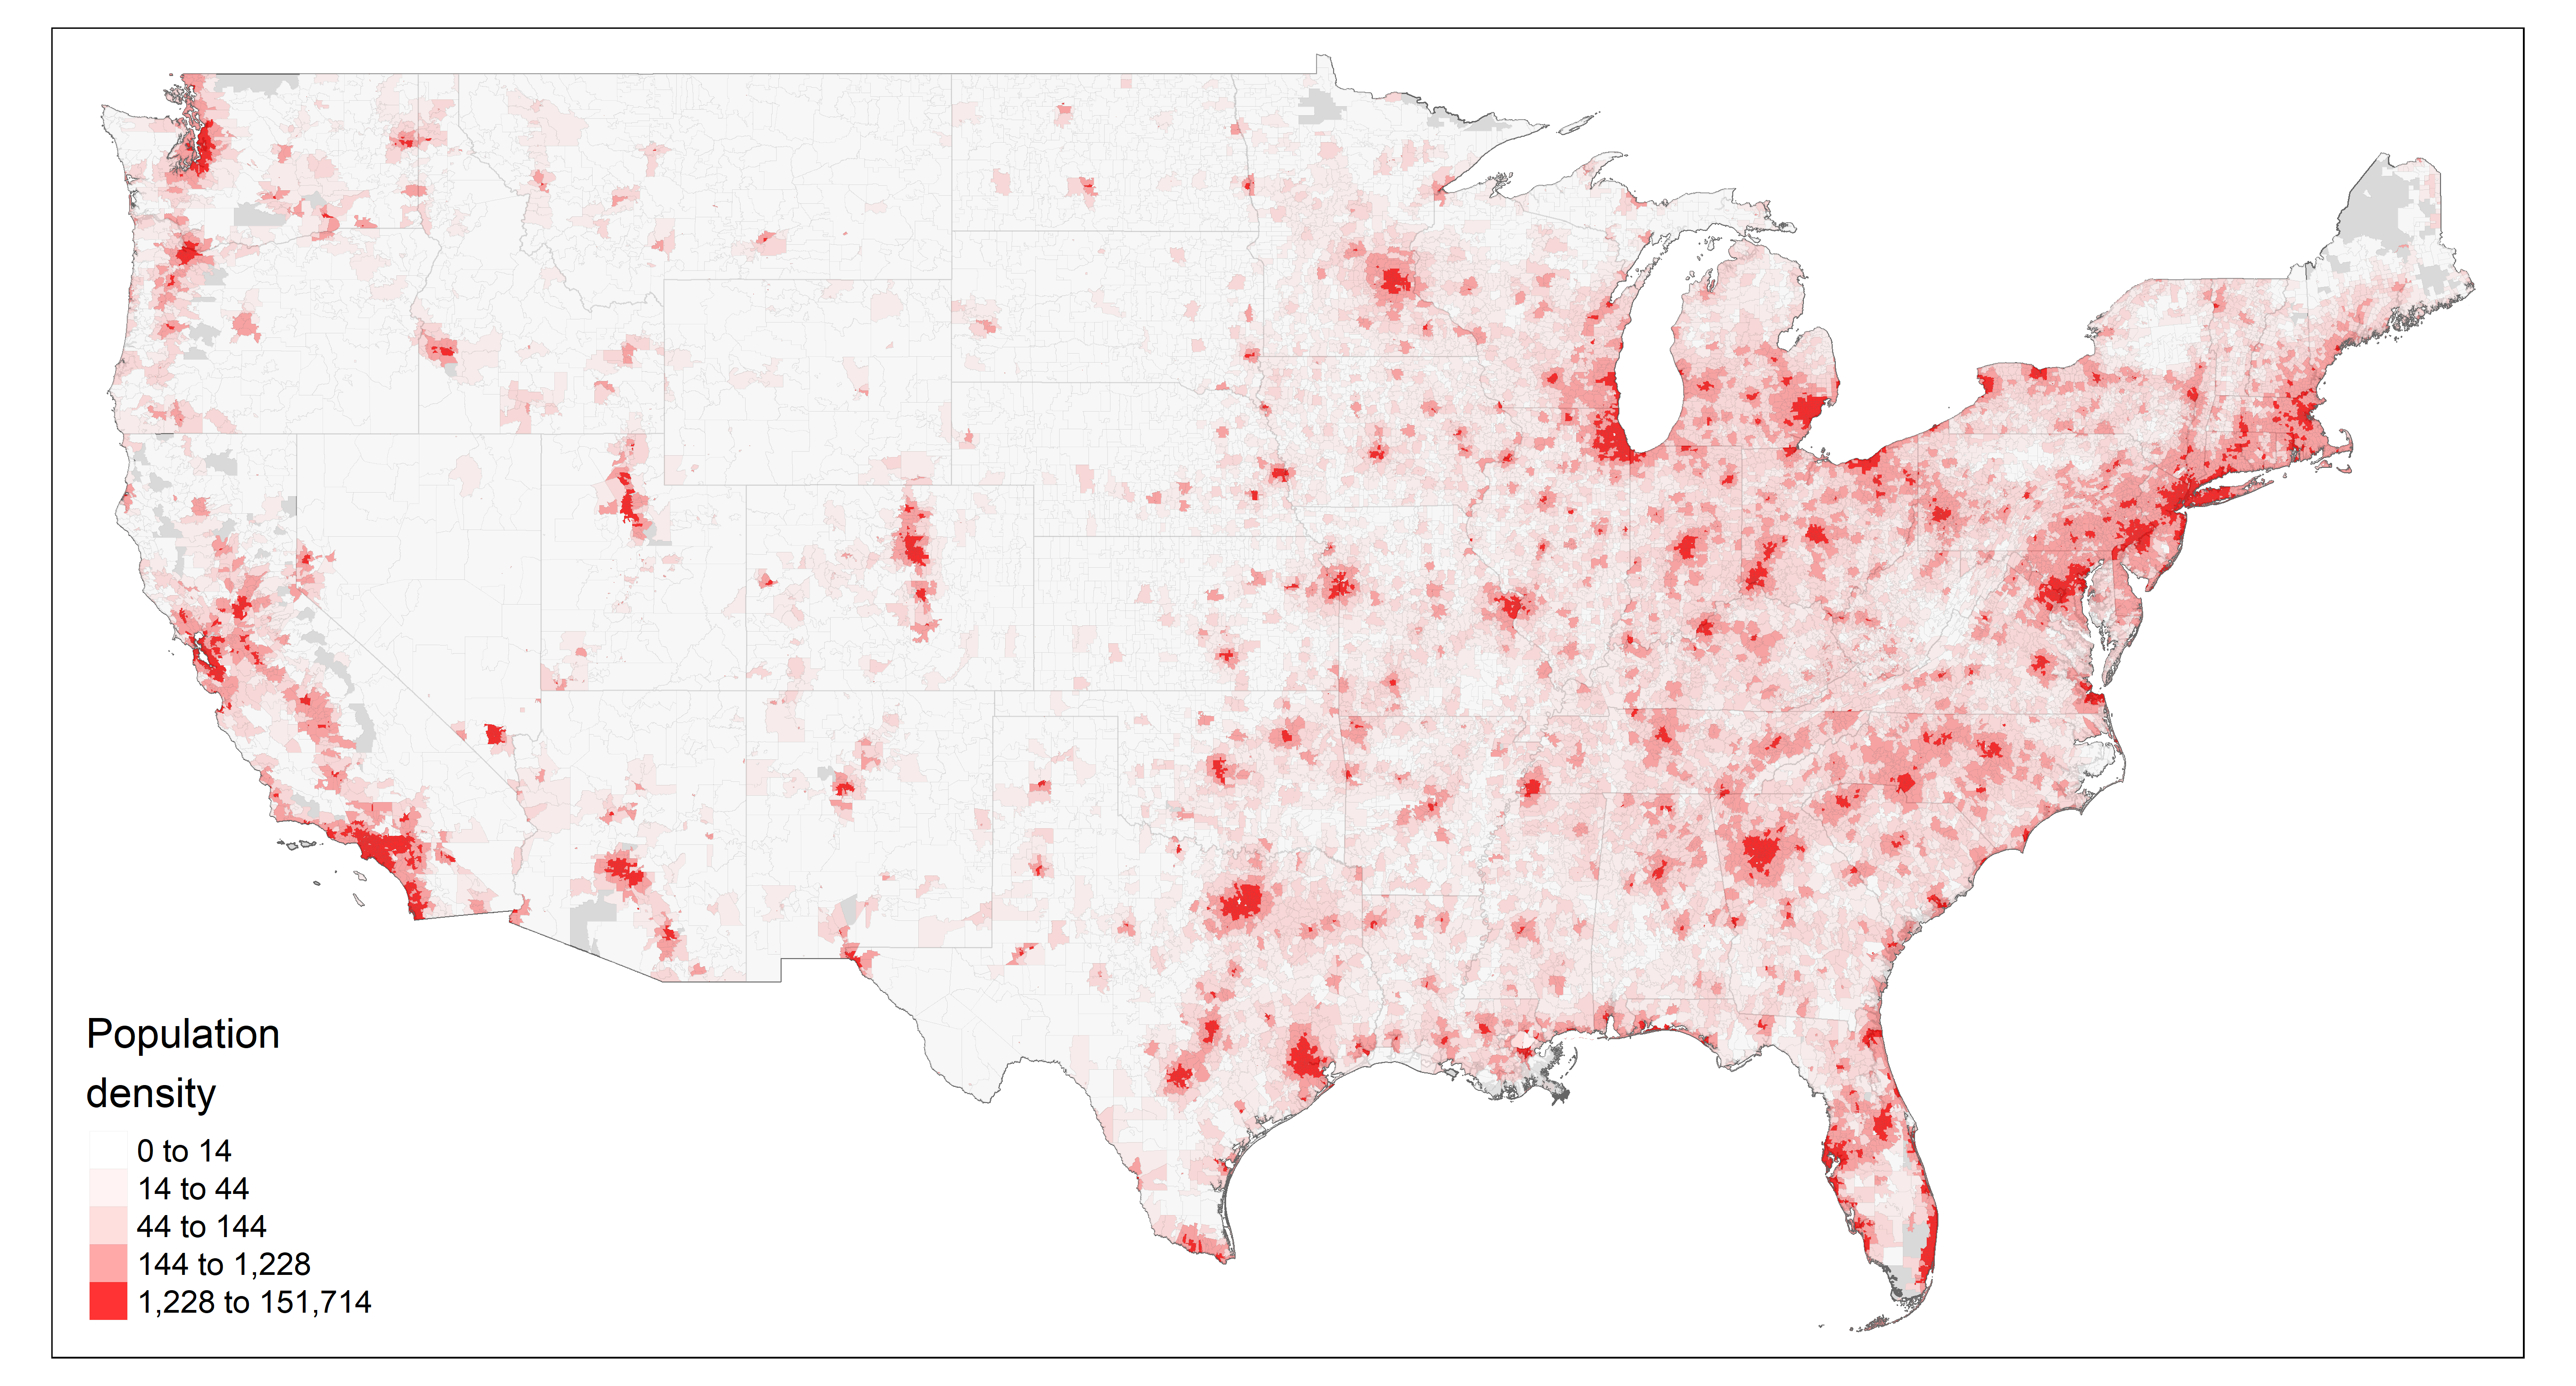
\includegraphics[width = 0.95\textwidth]
            {maps_US/output/USPS_zipcodes_pop_density.png}
    \end{subfigure}

    \begin{minipage}{.95\textwidth} \footnotesize
        \vspace{3mm}
        Notes:
        Data are from \textcite{ZillowData} and \textcite{ESRI}.
        The figure compares the USPS ZIP codes available in Zillow to the 
        population density.
        Panel (a) shows the sample of the ZIP codes that have rents data in 
        the SFCC category at any point in the period 2010--2019.
        Panel (b) shows quintiles of population density on 2020, measured in 
        population per square mile.
    \end{minipage}
\end{figure}
